\documentclass[dvipdfmx, tikz]{standalone}
\usepackage{tikz}
\usetikzlibrary{calc,decorations.pathreplacing,quotes,positioning,shapes,fit,arrows,backgrounds,tikzmark}

\begin{document}
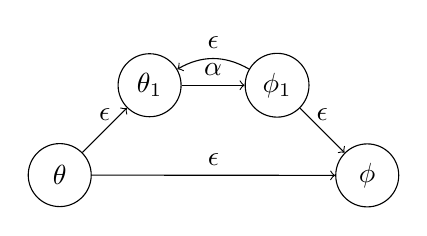
\begin{tikzpicture}[state/.style={circle, draw, minimum size=.8cm}, node distance=.8cm]
	\node(a0) [state] at (0,0) {$\theta$};
	\node(a1) [state, above right =of a0] {$\theta_1$};
	\node(a2) [state, right =of a1] {$\phi_1$};
	\node(a3) [state, below right =of a2] {$\phi$};
	
  \draw [->] (a0) to node(e0)[midway, above] {$\epsilon$} (a1);
  \draw [->] (a1) to node(e1)[midway, above] {$\alpha$} (a2);
  \draw [->] (a2) to node(e2)[midway, above] {$\epsilon$} (a3);
  \draw [->] (a0) to node(e3)[midway, above] {$\epsilon$} (a3);
  \draw [->] (a2) to [bend right] node(e4)[midway, above] {$\epsilon$} (a1);
  \ifx\TNFAActivateEdgeLabel\undefined \else
    \node[left=.0 of e0] {{\footnotesize $p\mathchar`-edge$}};
    \node[below=.0 of e1] {{\footnotesize $\alpha\mathchar`-edge$}};
    \node[right=.0 of e2] {{\footnotesize $p\mathchar`-edge$}};
    \node[below=.0 of e3] {{\footnotesize $p\mathchar`-edge$}};
    \node[above=.0 of e4] {{\footnotesize $b\mathchar`-edge$}};
  \fi

\end{tikzpicture}
\end{document}
